\documentclass[../main.tex]{subfiles}

\begin{document}

\clearpage

\subsection{Ejemplo teorico-práctico}

Siguiendo un ejemplo práctico, siguiendo la estructura mostrada en \cref{fig:real}

\begin{figure}[ht]
\centering
\begin{subfigure}{.5\textwidth}
  \centering
  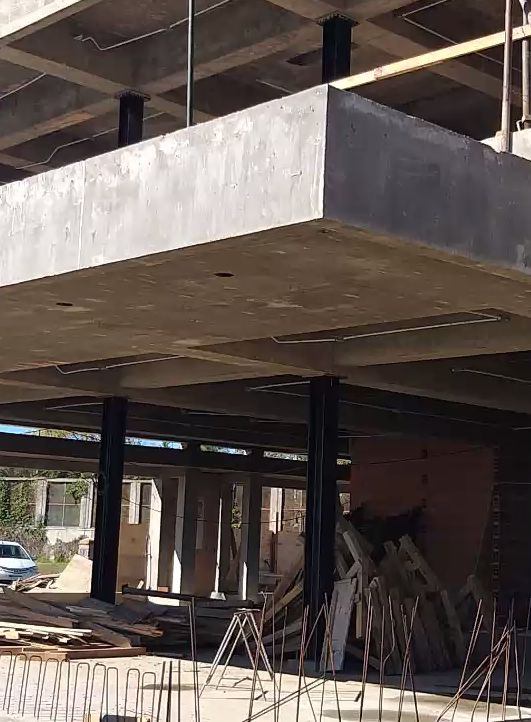
\includegraphics[width=.4\linewidth]{../images/20210426/ej1}
  \caption{A subfigure}
  \label{fig:sub1}
\end{subfigure}%
\begin{subfigure}{.5\textwidth}
  \centering
  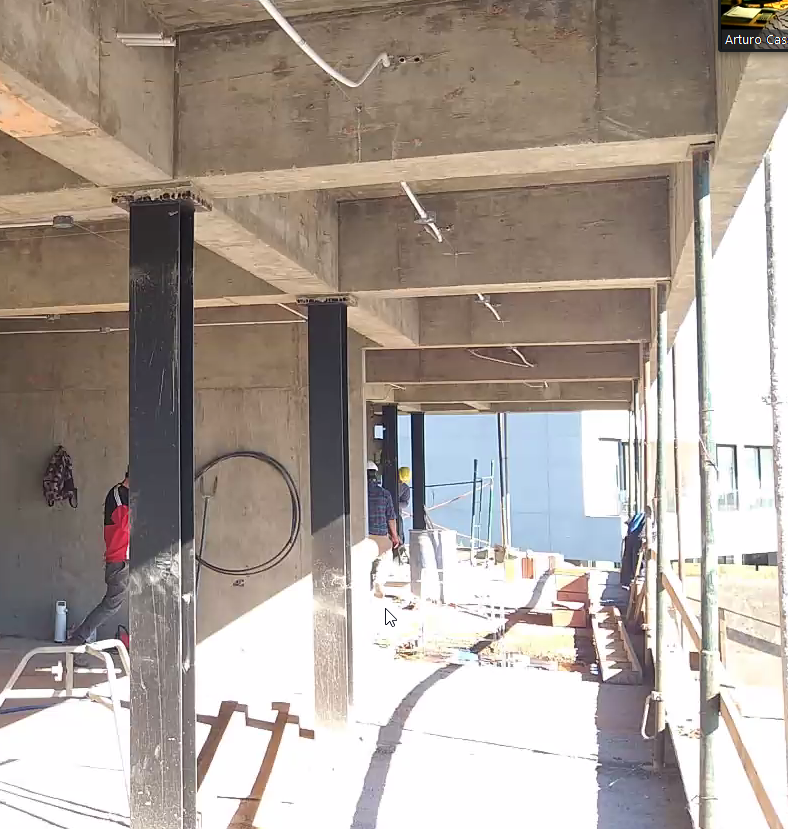
\includegraphics[width=.4\linewidth]{../images/20210426/ej2}
  \caption{A subfigure}
  \label{fig:sub2}
\end{subfigure}
\caption{Fotos reales de la estructura}
\label{fig:real}
\end{figure}

\begin{figure}[ht]
  \centering
  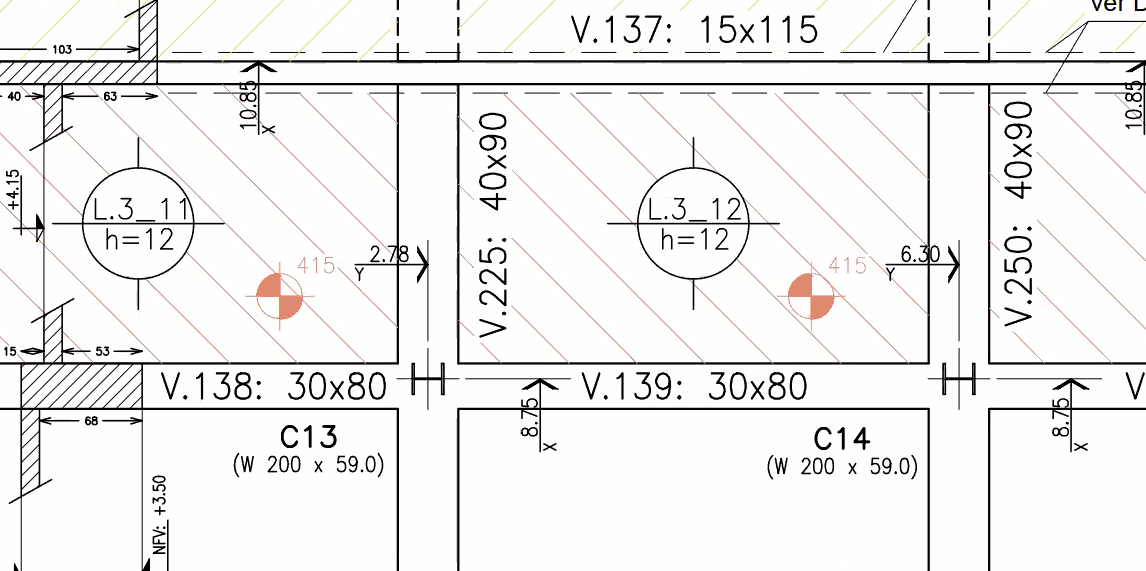
\includegraphics[width=0.8\textwidth]{../images/20210426/plano}
  \caption{Plano a calcular}
  \label{fig:plano}
\end{figure}

Consideramos una estructura como la siguiente:


%\begin{figure}[h]
%  \centering{
%  \resizebox{0.5\textwidth}{!}{%LaTeX with PSTricks extensions
%%Creator: Inkscape 1.0.2-2 (e86c870879, 2021-01-15)
%%Please note this file requires PSTricks extensions
\psset{xunit=.5pt,yunit=.5pt,runit=.5pt}
\begin{pspicture}(793.7007874,1122.51968504)
{
\newrgbcolor{curcolor}{0 0 0}
\pscustom[linewidth=0.87059526,linecolor=curcolor]
{
\newpath
\moveto(129.12234709,601.15067717)
\lineto(224.7129222,601.15067717)
}
}
{
\newrgbcolor{curcolor}{0 0 0}
\pscustom[linewidth=0.99999871,linecolor=curcolor]
{
\newpath
\moveto(173.16407811,601.0255748)
\lineto(173.16407811,892.30154835)
}
}
{
\newrgbcolor{curcolor}{0 0 0}
\pscustom[linewidth=0.78173482,linecolor=curcolor]
{
\newpath
\moveto(136.3792252,892.30154835)
\lineto(213.45225071,892.30154835)
}
}
{
\newrgbcolor{curcolor}{0 0 0}
\pscustom[linewidth=0.99999871,linecolor=curcolor]
{
\newpath
\moveto(173.16407811,601.0255748)
\lineto(157.12658646,586.02440315)
}
}
{
\newrgbcolor{curcolor}{0 0 0}
\pscustom[linewidth=0.99999871,linecolor=curcolor]
{
\newpath
\moveto(187.08642898,601.0255748)
\lineto(171.04893732,586.02440315)
}
}
{
\newrgbcolor{curcolor}{0 0 0}
\pscustom[linewidth=0.99999871,linecolor=curcolor]
{
\newpath
\moveto(201.3585789,601.0255748)
\lineto(185.32108724,586.02440315)
}
}
{
\newrgbcolor{curcolor}{0 0 0}
\pscustom[linewidth=0.99999871,linecolor=curcolor]
{
\newpath
\moveto(215.28092976,601.0255748)
\lineto(199.24343811,586.02440315)
}
}
{
\newrgbcolor{curcolor}{0 0 0}
\pscustom[linewidth=0.99999871,linecolor=curcolor]
{
\newpath
\moveto(141.95304945,601.0255748)
\lineto(125.9155578,586.02440315)
}
}
{
\newrgbcolor{curcolor}{0 0 0}
\pscustom[linewidth=0.99999871,linecolor=curcolor]
{
\newpath
\moveto(155.87540031,601.0255748)
\lineto(139.83790866,586.02440315)
}
}
{
\newrgbcolor{curcolor}{0 0 0}
\pscustom[linewidth=0.99999871,linecolor=curcolor]
{
\newpath
\moveto(189.20156976,907.30272)
\lineto(173.16407811,892.30154835)
}
}
{
\newrgbcolor{curcolor}{0 0 0}
\pscustom[linewidth=0.99999871,linecolor=curcolor]
{
\newpath
\moveto(203.12392063,907.30272)
\lineto(187.08642898,892.30154835)
}
}
{
\newrgbcolor{curcolor}{0 0 0}
\pscustom[linewidth=0.99999871,linecolor=curcolor]
{
\newpath
\moveto(217.39607055,907.30272)
\lineto(201.3585789,892.30154835)
}
}
{
\newrgbcolor{curcolor}{0 0 0}
\pscustom[linewidth=0.99999871,linecolor=curcolor]
{
\newpath
\moveto(157.9905411,907.30272)
\lineto(141.95304945,892.30154835)
}
}
{
\newrgbcolor{curcolor}{0 0 0}
\pscustom[linewidth=0.99999871,linecolor=curcolor]
{
\newpath
\moveto(171.91289197,907.30272)
\lineto(155.87540031,892.30154835)
}
}
{
\newrgbcolor{curcolor}{0.52941179 0.52941179 0.52941179}
\pscustom[linewidth=0.78173482,linecolor=curcolor]
{
\newpath
\moveto(213.45225071,892.30154835)
\lineto(290.52527622,892.30154835)
}
}
{
\newrgbcolor{curcolor}{0.52941179 0.52941179 0.52941179}
\pscustom[linewidth=0.99999871,linecolor=curcolor]
{
\newpath
\moveto(266.27459528,907.30272)
\lineto(250.23710362,892.30154835)
}
}
{
\newrgbcolor{curcolor}{0.52941179 0.52941179 0.52941179}
\pscustom[linewidth=0.99999871,linecolor=curcolor]
{
\newpath
\moveto(280.19694614,907.30272)
\lineto(264.15945449,892.30154835)
}
}
{
\newrgbcolor{curcolor}{0.52941179 0.52941179 0.52941179}
\pscustom[linewidth=0.99999871,linecolor=curcolor]
{
\newpath
\moveto(294.46909606,907.30272)
\lineto(278.43160441,892.30154835)
}
}
{
\newrgbcolor{curcolor}{0.52941179 0.52941179 0.52941179}
\pscustom[linewidth=0.99999871,linecolor=curcolor]
{
\newpath
\moveto(235.06356661,907.30272)
\lineto(219.02607496,892.30154835)
}
}
{
\newrgbcolor{curcolor}{0.52941179 0.52941179 0.52941179}
\pscustom[linewidth=0.99999871,linecolor=curcolor]
{
\newpath
\moveto(248.98591748,907.30272)
\lineto(232.94842583,892.30154835)
}
}
{
\newrgbcolor{curcolor}{0.52941179 0.52941179 0.52941179}
\pscustom[linewidth=0.99999871,linecolor=curcolor]
{
\newpath
\moveto(173.16407811,601.15067717)
\curveto(164.01630614,707.02601575)(208.15909417,807.44192126)(250.23710362,892.30154835)
}
}
\end{pspicture}
}}
%  \caption{your caption} \label{fig:figureone}
%\end{figure}


Entonces, tenemos que considerar un $k=1.2$. 
Consideramos una altura desde $h = \SI{2.8}{m}$, con un, y tenemos un perfil
\textbf{W200.59}, que vamos a considerar como el \textbf{W8x40} que se encuentra
en el reglamento CIRSOC. El perfil tendrá un $f_y = \SI{345}{MPa} $ y  
$f_u = \SI{450}{MPa}$.

Desarrollo:

\begin{align*}
  \lambda &= \frac{1}{\pi} * \frac{k*L}{r} * \sqrt{\frac{f_y}{E}} \\[5pt] 
  \lambda &=   \frac{1}{\pi} * \frac{1*280}{5.18} * \sqrt{\frac{355}{200000}} \\[5pt]
  \lambda &= 0.8698
.\end{align*}

Entonces podemos obtener los valores de $F_{cr}$ de la siguiente forma:

\begin{align*}
  f_{cr} &= 0.658^{0.8698^2} * F_y\\[5pt] 
  f_{cr} &= \SI{258.6}{MPa}
.\end{align*}

Conseguimos entonces los valores de tensión y carga critica como:

\begin{align*}
  P_d &= \phi * f_{cr} * A \\[5pt]
  P_d &= \SI{1660}{kN} 
.\end{align*}

\subsubsection{Recordatorio}

Es necesario acordarse de que cuando $\lambda\leq 1.5$ se utiliza:

\begin{align*}
  F_{cr} = 0.658^{\lambda^2}*F_y
.\end{align*}

Y cuando se da que $\lambda\geq 1.5$ tenemos que considerar:

\begin{align*}
  F_{cr} = \frac{0.877}{\lambda^2}*F_y
.\end{align*}

\end{document}
